\documentclass{beamer}
\usetheme{Boadilla}
\usepackage{graphicx}

\title{Call Thesis - 22/05/2019}
\author{Matteo Avigni}
\begin{document}
\begin{frame}[plain]
    \maketitle
\end{frame}
\begin{frame}{Agenda}
	\begin{itemize}		
		\item Dataset: sfruttare il lavoro di Marcello e integrarlo con quello di Samuele
		\item Distribuzione rendimenti
	\end{itemize}
\end{frame}


\begin{frame}{BTC returns}
	\begin{figure}	
		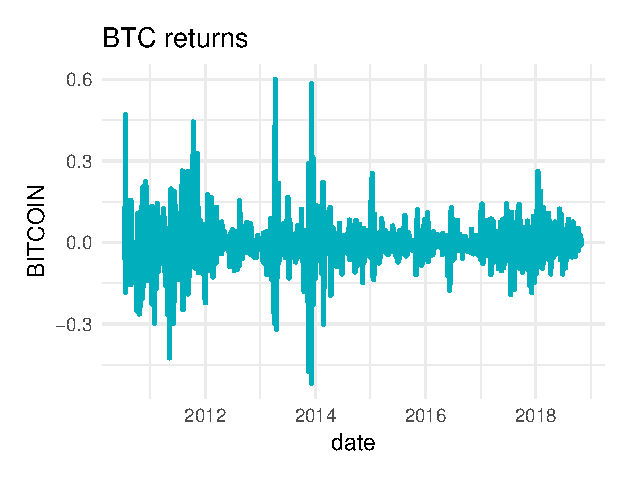
\includegraphics[width=120mm]{BTCreturns.eps}
	\end{figure}
\end{frame}
\begin{frame}{BTC returns qqplot}
	\begin{figure}[linewidth=250mm]	
		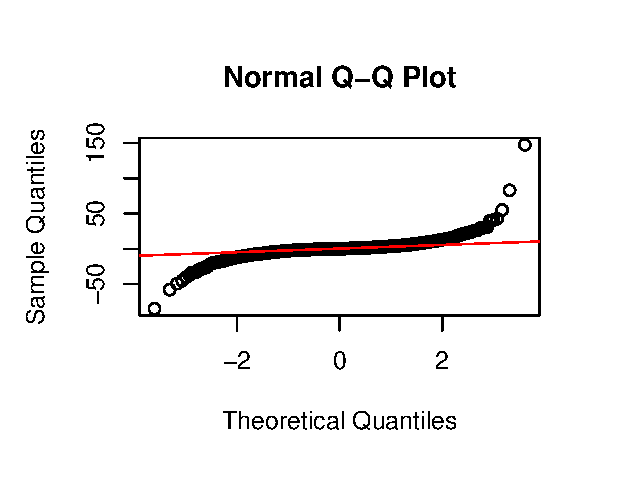
\includegraphics[width=110mm]{BTCqqplot.eps}
	\end{figure}
\end{frame}
%\begin{frame}{SPX returns qqplot}
%	\begin{figure}[b]	
%		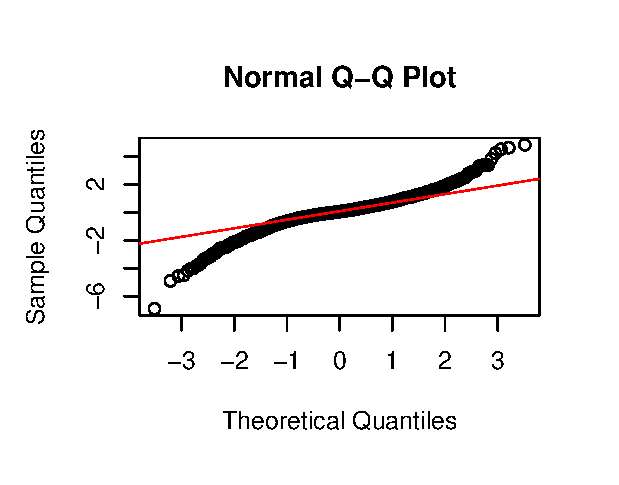
\includegraphics{SPXqqplot.eps}
%	\end{figure}
%\end{frame}

\begin{frame}{BTC returns lagplot}
	\begin{figure}[linewidth=250mm]	
		\includegraphics[width=110mm]{lagplot.eps}
	\end{figure}
\end{frame}


\begin{frame}{BTC returns autocorrelation}
	\begin{figure}[linewidth=250mm]	
		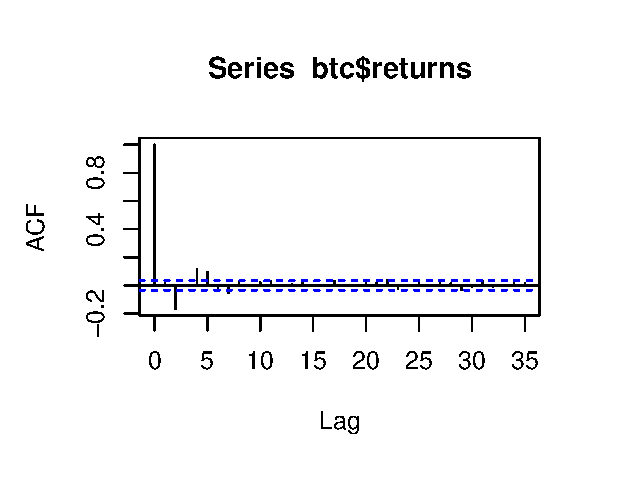
\includegraphics[width=110mm]{BTCautocor.eps}
	\end{figure}
\end{frame}


\begin{frame}{BTC returns absolute value autocorrelation}
	\begin{figure}[b]	
		\includegraphics[width=104mm]{BTCabsret.eps}
	\end{figure}
\end{frame}

%\begin{frame}
%	\begin{center}
%		\begin{tabular}{l|*{3}{c}r}
%		\multicolumn{4}{c}{Ljung-Box}\\
%				& Xsquared & df & p-value \\
%		\hline
%			BTC & 195.78 & 25 & 2.2e-16 \\  
%			SPX & 71.285 & 25 & 2.476e-06  
%		\end{tabular}
%
%		\bigskip
%		\bigskip
%		\begin{tabular}{l|*{3}{c}r}
%			\multicolumn{4}{c}{Augmented Dickey–Fuller (ADF) t-statistic test}\\
%				& Dickey-Fuller & Lag order & p-value \\
%			\hline
%			BTC & -13.507 & 14 & 0.01 \\  
%			SPX & -14.538 & 13 & 0.01  
%		\end{tabular}
%	\end{center}
%\end{frame}

\begin{frame}{Conclusioni}
	\begin{itemize}
		\item Test di ipotesi sulla stazionarietà
		\item ARIMA, GARCH
		\item Extreme value theory?
	\end{itemize}
\end{frame}





\end{document}
